\documentclass[10pt, margin=1mm,convert={density=500,outext=.png}]{standalone}
\usepackage{cmbright}
\usepackage[OT1]{fontenc}
\usepackage{graphicx}
\usepackage{amsmath}
\usepackage{tabularx}
\usepackage{booktabs}
\usepackage[table]{xcolor}
\usepackage{colortbl}
\usepackage{braket}
\usepackage{adjustbox}
\usepackage{multirow}
\usepackage{dsfont}
\usepackage{makecell}

\graphicspath{ {../} }

% \newcommand{\toprule}{\hline}
% \newcommand{\bottomrule}{\hline}
% \newcommand{\midrule}{\hline}
% \newcommand{\cmidrule}[#1]{\cline{#1}}

% Try out cell padding to handle fractions
% Must prefix column formatters with `S'
\usepackage{cellspace}
\setlength\cellspacetoplimit{4pt}
\setlength\cellspacebottomlimit{4pt}

\definecolor{Gray}{gray}{0.95}
\newcolumntype{a}{>{\columncolor{Gray}}c}

\renewcommand{\familydefault}{\sfdefault}

% \setlength{\tabcolsep}{12pt}

\begin{document}
\small

\begin{tabular}{ccccc}
% \multicolumn{4}{c}{How to construct a reduced-order model for the eigenvalue problem}
% \\[2pt]
\toprule
\multirowcell{2}{
High-fidelity system
}
% High-fidelity system
% \multirow{2}{*}{\shortstack[l]{{High-fidelity system\\ Eigenvalue problem}}
% \multicolumn{1}{|c|}{High-fidelity system}
% \multicolumn{1}{|c|}{\multirowcell{2}{High-fidelity system\\ Eigenvalue problem}}
% \multirowcell{2}{
% \multirow{2}{*}{
% \begin{tabularx}{\cellwidth}{|c|}
% High-fidelity system\\ Eigenvalue problem
% \end{tabularx}
% }
& \multicolumn{3}{c}{Constructing a reduced-order model for bound states}\\
% \cmidrule(lr){1-1}
\cmidrule(lr){2-4}
% &
% High-fidelity system & \multicolumn{2}{c}{Offline Phase} & Online Phase\\
% Eigenvalue problem
% \multicolumn{1}{|c|}{Eigenvalue problem}
% \multicolumn{1}{|c|}{}
& \multicolumn{2}{c}{Offline stage} & Online stage \\
% \cmidrule(lr){3-4}\cmidrule(lr){5-5}
% \cmidrule(lr){1-1}
\cmidrule(lr){1-1}
\cmidrule(lr){2-3}\cmidrule(lr){4-4}

% &
\hspace{0.45in}$H(\boldsymbol{\theta})\hspace{0.43in}\ket{\psi}\hspace{0.05in}=E\hspace{0.06in}~\ket{\psi}$~
%\!\!
&
\!\!\!\!Snapshots $\psi(\boldsymbol{\theta}_i)$\!\!\!\!\!\!\!\!%\!\!
& Projection (after orthonormalizing snapshots)
& Emulation ($E \approx \widetilde E$)
\\[2pt]

% Steps
% &

% \multirow[b]{2}{*}{
$
\!\!
\begin{bmatrix}
\vcenter{\hbox{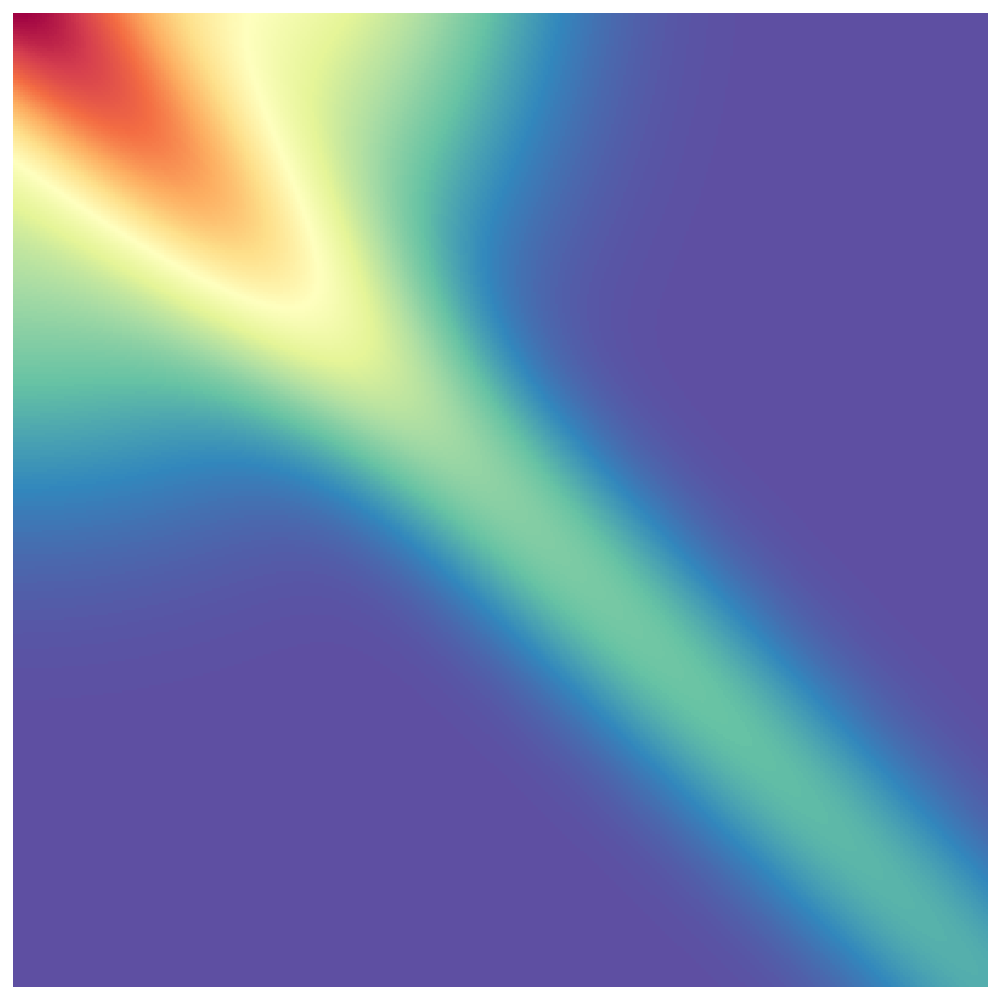
\includegraphics{highfidelity.png}}}
\end{bmatrix}
\!\!
\begin{bmatrix}
\vcenter{\hbox{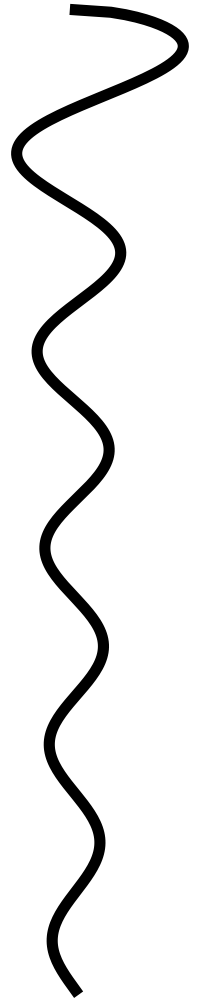
\includegraphics{wave_function.png}}}
\end{bmatrix}
\!\!
=
E
\begin{bmatrix}
\vcenter{\hbox{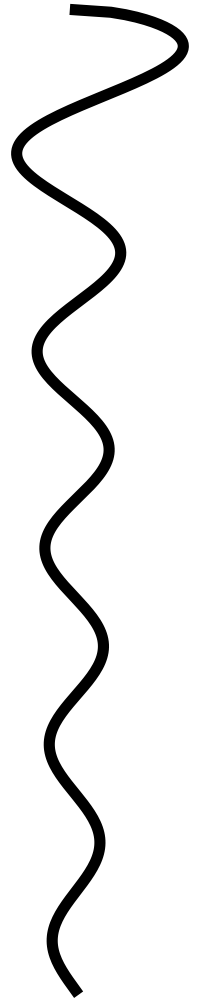
\includegraphics{wave_function.png}}}
\end{bmatrix}
%\!\!%\!\!
$
% }

&

% \multirow[b]{2}{*}{
$
% X =
\begin{bmatrix}
\vcenter{\hbox{
\includegraphics{basis.png}}}
\end{bmatrix}
$
% }

&

% \multirow[c]{2}{*}{
$
\!\!\!\!\!\!
\begin{bmatrix}
\vcenter{\hbox{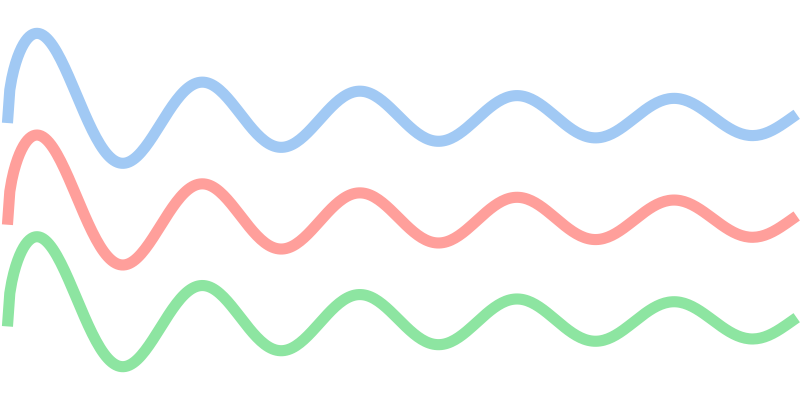
\includegraphics{basis_t.png}}}
\end{bmatrix}
\!\!
\begin{bmatrix}
\vcenter{\hbox{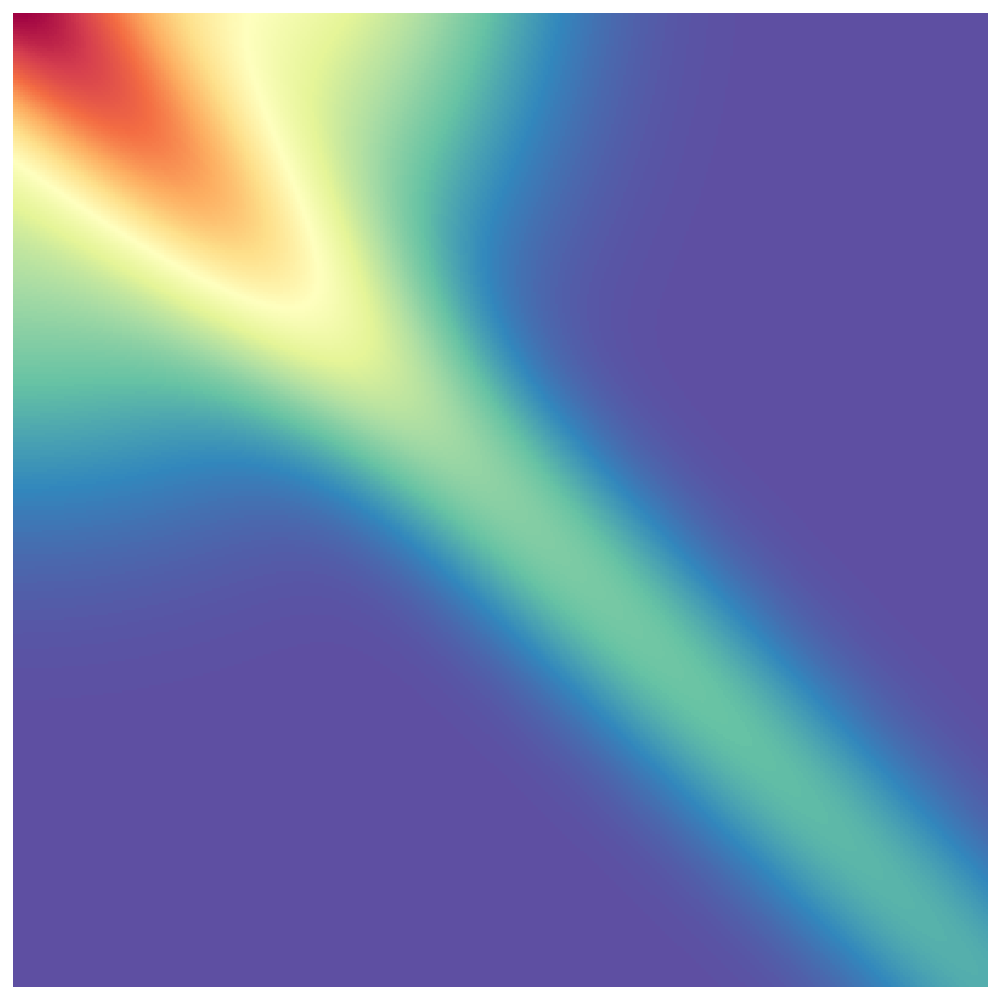
\includegraphics{highfidelity.png}}}
\end{bmatrix}
\!\!
\begin{bmatrix}
\vcenter{\hbox{
\includegraphics{basis.png}}}
\end{bmatrix}
\!\!
% \longrightarrow
=
\!\!
\begin{bmatrix}
\vcenter{\hbox{
\includegraphics{projected_matrix.png}}}
\end{bmatrix}
$
% }

&

% \adjustbox{valign=t,minipage=4cm}{%
% \vspace{-1in}
% \vspace{-10cm}
{
% \vspace{-1in}
% \rule{0pt}{-1in}
% \begin{minipage}[t]{\textwidth}
% test
$
\begin{aligned}
\widetilde H(\boldsymbol{\theta}) ~~~~\vec{\beta}~ & = \widetilde E\widetilde N \vec{\beta} \\
\begin{bmatrix}
\vcenter{\hbox{
\includegraphics{projected_matrix.png}}}
\end{bmatrix}
\!\!
\begin{bmatrix}
\vcenter{\hbox{
\includegraphics{coefficients.png}}}
\end{bmatrix}
\!\!
 & =
\widetilde E
\begin{bmatrix}
\vcenter{\hbox{
\includegraphics{coefficients.png}}}
\end{bmatrix}
\\
% \phantom{H \vec{\beta} = \widetilde E \vec{\beta}}
(\widetilde N & = \mathds{1})
\!\!
\end{aligned}
% % \rule{0pt}{-1in} 
$
}
% \vspace{10cm}
% \end{minipage}
% \vtop{\null\hbox{test}}
% \raisebox{-\height+\baselineskip}{test}

% \vspace{-1cm}
% test
% \vspace{1cm}
% \begin{tabular}[t]{l} first \\ second \end{tabular}
% }

% \\

% & & & hi

\\[32pt]

\multicolumn{1}{l}{\hspace{0.35in}$N_h \times N_h$\hspace{0.43in}$N_h$\hspace{0.47in}$N_h$}
& $N_h \times n_b$
&
\multicolumn{1}{r}{$n_b \times N_h$\hspace{0.62in}$N_h \times N_h$\hspace{0.36in}$N_h \times n_b$\hspace{0.19in}$n_b \times n_b\hspace{0.06in}$}
&
% $n_b \times n_b$\hspace{0.6in}
All size-$n_b$ operations

\\
% \midrule
\cmidrule(lr){1-4}

% Time
% $t$
% &
Time:~
$\vcenter{\hbox{
\includegraphics{time_long.png}}}$ per $\theta$ sample &

\!\!\!$n_b \times \vcenter{\hbox{
\includegraphics{time_long.png}}}$\!%\!\!

&

$\sim \vcenter{\hbox{
\includegraphics{time_long.png}}}$

&


% \!\!\!\!%
% Sampling $\theta$: $\vcenter{\hbox{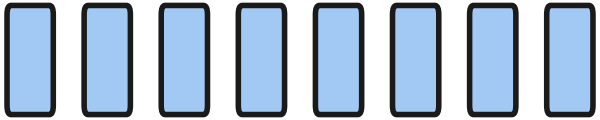
\includegraphics{time_short.png}}}$
% \!\!\!\!%
% \!\!\!\!%
$\vcenter{\hbox{
\includegraphics{time_short_individual.png}}}$ per $\theta$ sample
% \!\!\!\!%
\\
\bottomrule
\\[-8pt]
& & &
\multicolumn{1}{r}{
\hspace{-4in}%
CPU time scales with the length of $\vcenter{\hbox{
\includegraphics{time_long.png}}}$
}
\end{tabular}
\end{document}
